\documentclass{article}
\usepackage[left=1in,top=2in,bottom=1in,right=1in]{geometry}
\usepackage{listings}
\usepackage{graphicx}
\usepackage{hyperref}
\usepackage{breakurl}
\usepackage{subfigure}

\newcommand{\theurl}{\texttt{video.cs.cmu.edu}}

\title{	15-441: Computer Networks\\
Project 3: Video CDN\\
}
\author{\textbf{Lead TAs:}\\ 
             Matt Mukerjee
             $<$\href{mailto:mukerjee@cs.cmu.edu}{mukerjee@cs.cmu.edu}$>$\\
			 David Naylor
             $<$\href{mailto:dnaylor@cs.cmu.edu}{dnaylor@cs.cmu.edu}$>$}
\date{}
\begin{document}
\maketitle

\large{\noindent \textbf{Assigned: 11/7/13\\
Checkpoint 1 due: 11/21/13 (11:59 PM)\\
Final version due: 12/5/13 (11:59 PM)}}


\section{Overview}

In this project you will explore how video content distribution networks (CDNs)
work. In particular, you will implement adaptive bitrate selection, DNS load
balancing, and pieces of OSPF (which your DNS server will use to decide which
server is closest to a given client).

\subsection{In the Real World}

Figure~\ref{fig:overview-real} depicts (at a high level) what this system looks
like in the real world. Clients trying to stream a video first issue a DNS
query to resolve the service's domain name to an IP address for one of the
CDN's content servers. The CDN's authoritative DNS server selects the ``best''
content server for each particular client based on (1) the client's IP address
(from which it learns the client's geographic location) and (2) current load on
the content servers (which the servers periodically report to the DNS server).

Once the client has the IP address for one of the content servers, it begins
requesting chunks of the video the user requested. The video is encoded at
multiple bitrates; as the client player receives video data, it calculates the
throughput of the transfer and requests the highest bitrate the connection can
support.

\begin{figure}
	\centering
	\begin{minipage}{0.4\textwidth}
		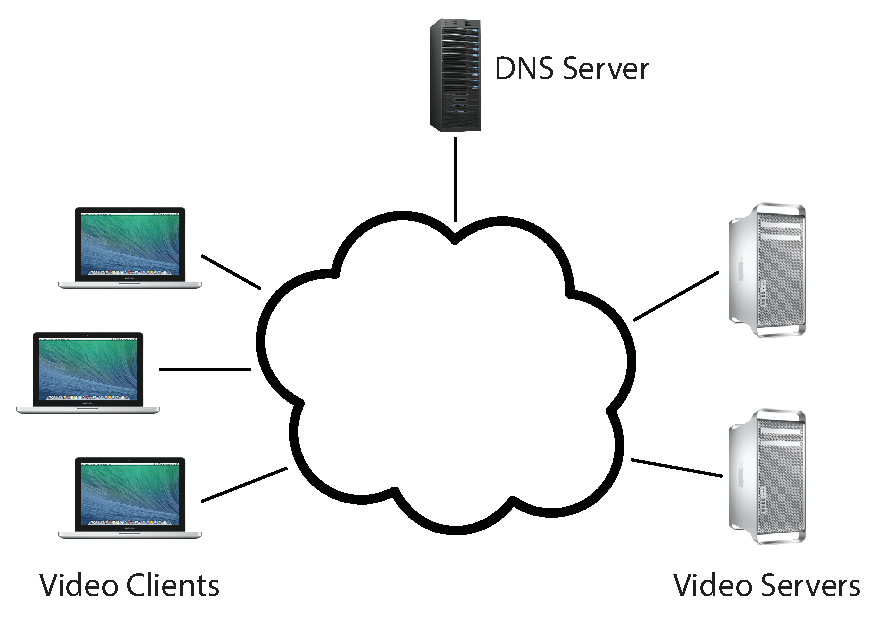
\includegraphics[width=\columnwidth]{figs/overview-real.eps}
		\caption{In the real world...}
		\label{fig:overview-real}
	\end{minipage}
	\hfill
	\begin{minipage}{0.4\textwidth}
		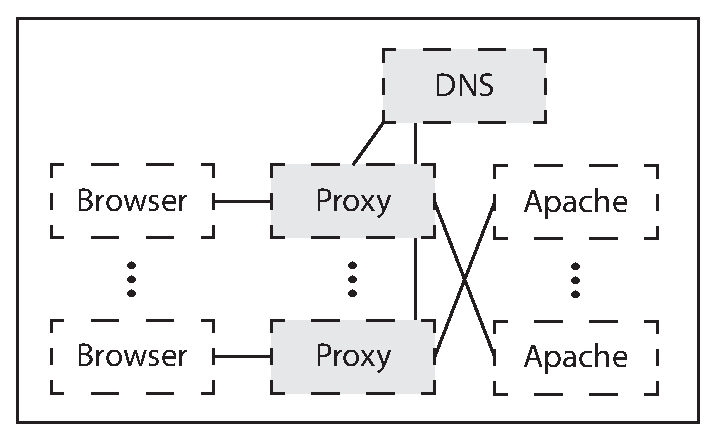
\includegraphics[width=\columnwidth]{figs/overview-fake.eps}
		\caption{Your system.}
		\label{fig:overview-fake}
	\end{minipage}

	\caption{System overview.}
	\label{fig:overview}
\end{figure}

\subsection{Your System}

Implementing an entire CDN is clearly a tall order, so let's simplify things.
First, your entire system will run on one host; we're providing a network
simulator (described in \S\ref{sec:starter}) that will allow you to run several
processes with arbitrary IP addresses on one machine. Our simulater also allows
you to assign arbitrary link characteristics (bandwidth and latency) to each
pair of ``endhosts'' (processes). For this project, you will do your
development and testing using a virtual machine we provide
(\S\ref{sec:starter}).

Figure~\ref{fig:overview-fake} shows the pieces of the system; those shaded in
gray will be written by you.

\medskip\noindent \textbf{Browser.} You'll use an off-the-shelf web browser to play
videos served by your CDN. Requests should be sent via a proxy (see below); you
can specify an HTTP proxy in your browser's preferences, though we recommended
using the FoxyProxy plugin for Firefox (which allows you to select from many
proxies based on URL patterns).

\medskip \noindent \textbf{Proxy.} Rather than modify the video player itself, you will
implement adaptive bitrate selection in an HTTP proxy. The player requests
chunks with standard HTTP GET requests; your proxy will intercept these and
modify them to retrieve whichever bitrate your algorithm deems appropriate. To
simulate multiple clients, you will launch multiple instances of your proxy
(each one binding to a different fake IP address). More detail in
\S\ref{sec:proxy}.

\medskip \noindent \textbf{Web Server.} Video content will be served from an
off-the-shelf web server (Apache). As with the proxy, you will run multiple
instances of Apache on different fake IP addresses to simulate a CDN with
several content servers. More detail in \S\ref{sec:starter}.

\medskip \noindent \textbf{DNS Server.} You will implement a simple DNS (supporting only
a small portion of actual DNS functionality). Your server will respond to each
request with the ``best'' server for that particular client. More detail in
\S\ref{sec:dns}.




\section{Video Bitrate Adaptation}
\label{sec:proxy}

Many video players monitor how quickly they receive data from the server and
use this throughput value to request better or lower quality encodings of the
video, aiming to stream the highest quality encoding that the connection can
handle. Rather than modifying an existing video client to perform bitrate
adaptation, you will implement this functionality in an HTTP proxy through
which your browser will direct reqeusts.


\subsection{Requirements}

\bigskip \noindent \textbf{Checkpoint 1:}~~For the first checkpoint, your proxy
should simply accept requests from the video player, resolve the server's
hostname to an IP address, forward the requests to the server, and return the
server's responses to the player. For this checkpoint you do not need to worry
about throughput measurement or bitrate adaptation.

\textbf{TODO: need to handle multiple simultaneous connections?}


\bigskip \noindent \textbf{Checkpoint 2:}~~For the final submission, your proxy
should calculate the throughput it receives from the video server and select
the best bitrate for the connection. See \S\ref{sec:proxy-details} for details.


\subsection{Implementation Details}
\label{sec:proxy-details}

\subsubsection{Throughput Calculation}
Your proxy could estimate your connection's throughput once per chunk as
follows. Note the start time, $t_s$, of each chunk request (i.e., save a
timestamp when your proxy receives a request from the player). Save another
timestamp, $t_f$, when you have finished receiving the chunk from the server.
Now, given the size of the chunk, $B$, you can computer the throughput, $T$,
your proxy saw for this chunk:
\[
	T = \frac{B}{t_f - t_s}
\]


To smooth your current throughput estimation, your proxy should use an
exponentially-weighted moving average (EWMA). Every time you make a new
measurement ($T_{new}$), update your current throughput estimation as follows:
\[
	T_{current} = \alpha T_{new}  +  (1 - \alpha)T_{current}
\]
The constant $0 \leq \alpha \leq 1$ controls the tradeoff between a smooth
throughput estimate ($\alpha$ closer to 0) and one that reacts quickly to
changes ($\alpha$ closer to 1).

\textbf{TODO: how to pick $\alpha$?}



\subsubsection{Choosing a Bitrate}

Once your proxy has calculated the connection's current throughput, it should
select the highest offered bitrate the connection can support. Your proxy
should learn which bitrates are available for a given video by parsing the
manifest file (the ``.f4m'' initially requested at the beginning of the
stream). The manifest is encoded in XML; each encoding of the video is
described by a \texttt{$<$media$>$} element, whose \texttt{bitrate} attribute
you should find.

Your proxy replaces each chunk request with a request for the same chunk at the
selected bitrate (in Kbps) by modifying the HTTP request's Request-URI. Video
chunk URIs are structured as follows:
\begin{center}
	\texttt{/path/to/video/$<$video-name$>$-$<$bitrate$>$Seq$<$num$>$-Frag$<$num$>$}
\end{center}

For example, suppose the player requests fragment 3 of chunk 2 of the video Big
Buck Bunny at 500 Kbps:
\begin{center}
	\texttt{/path/to/video/big\_buck\_bunny\_480p\_h264-500Seq2-Frag3}
\end{center}
To switch to a higher bitrate, e.g., 1000 Kbps, the proxy should modify the URI
like this:
\begin{center}
	\texttt{/path/to/video/big\_buck\_bunny\_480p\_h264-1000Seq2-Frag3}
\end{center}


\subsubsection{Running the Proxy}

By running \texttt{make} in the root of your
submission directory, we should be able to create an executable called
\texttt{proxy}, which should be invoked as follows:
\begin{center}
	\texttt{./proxy $<$listen-ip$>$ $<$listen-port$>$ $<$dns-ip$>$ $<$dns-port$>$}
\end{center}

\begin{description}
	\item[\texttt{listen-ip}] The IP address your proxy should listen on.
	\item[\texttt{listen-port}] The TCP port your proxy should listen on.
	\item[\texttt{dns-ip}] IP address of the DNS server.
	\item[\texttt{dns-port}] UDP port DNS server listens on.
\end{description}





\section{DNS Load Balancing}
\label{sec:dns}

To spread the load of serving videos among a group of servers, most CDNs
perform some kind of load balancing. A common technique is to configure the
CDN's authoritative DNS server to resolve a single domain name to one out of a
set of IP addresses belonging to replicated content servers. The DNS server can
use various strategies to spread the load, e.g., round-robin, shortest
geographic distance, or current server load (which requires servers to
periodically report their statuses to the DNS server).

\subsection{Requirements}

You will write a simple DNS server that implements load balancing two different
ways: round-robin and geographic distance.

\bigskip \noindent \textbf{Checkpoint 1:}~~For the first checkpoint, you must
implement a simple round-robin based DNS load balancer. Your DNS process should
take as input a list of video server IP addresses (see \S\ref{sec:dns-details});
it responds to each request to resolve the name \theurl by returning the next
IP address in the list, cycling back to the beginning when the list is
exhausted.

In order for you proxy to be able to query your DNS server, you must also write
an accompanying DNS resolution library. (See \S\ref{sec:dns-details} for
details.)



\bigskip \noindent \textbf{Checkpoint 2:}~~~For the second checkpoint, you will
be somewhat more sophisticated. Now your DNS server must return the closest
video server to the client based on the client's IP address. In the real world,
this would be done by querying a database mapping IP prefixes to geographic
locations. In your implementation, you will pretend that a link state routing
protocol (e.g., OSPF) is used Internet-wide and that your DNS server
participates in it. Your DNS server must process link state advertisements
(LSAs), build a graph of the entire network, and run Dijkstra's shortest path
algorithm on the graph to determine the closest video server for a given
client.

\emph{You do not need to implement LSA flooding.} We will provide you with a
file containing a list of LSAs which your server would have received had you
actually implemented LSA flooding.  The file contains one LSA per line,
formatted as follows:
\begin{center}
	\texttt{$<$sender$>$ $<$sequence number$>$ $<$neighbors$>$}
\end{center}
The \texttt{sender} is the IP address of the node that originated this LSA. The
\texttt{sequence number} is an integer allowing you to order the LSAs from a
given sender (you may assume sequence numbers don't wrap back to zero within
the LSA file). \texttt{neighbors} is a comma-separated string of IP addresses
denoting the sender's immediate (directly connected) neighbors.

\textbf{Describe gotchas --- cite peterson
davie?} 


\subsection{Implementation Details}
\label{sec:dns-details}

Your DNS implementation will consist of two pieces: your DNS server and your
DNS resolution library. The two pieces should communicate using the DNS message
formats defined in section 4.1 of RFC 1035. To make your life easier:

\begin{description}
	\item[\texttt{AA}] Set this to 0 in requests, 1 in responses.
	\item[\texttt{RD}] Set this to 0 in all messages.
	\item[\texttt{RA}] Set this to 0 in all messages.
	\item[\texttt{Z}] Set this to 0 in all messages.
	\item[\texttt{NSCOUNT}] Set this to 0 in all messages.
	\item[\texttt{ARCOUNT}] Set this to 0 in all messages.
	\item[\texttt{QTYPE}] Set this to 1 in all requests (asking for an A record).
	\item[\texttt{QCLASS}] Set this to 1 in all requests (asking for an IP address).
	\item[\texttt{TYPE}] Set this to 1 in all responses (returning an A record).
	\item[\texttt{CLASS}] Set this to 1 in all responses (returning an IP address).
	\item[\texttt{TTL}] Set this to 0 in all responses (no caching).
\end{description}

\bigskip \noindent \textbf{Server.} Your DNS server will operate over UDP. It
will bind to an IP address and port specified as a command line arguments. It
need only respond to requests for \theurl; any other requests should generate a
response with \texttt{RCODE} 3. By running \texttt{make} in the root of your
submission directory, we should be able to create an executable called
\texttt{nameserver}, which should be invoked as follows \emph{even if not all
arguments are functional}:
\begin{center}
	\texttt{./nameserver [-r] $<$ip$>$ $<$port$>$ $<$servers$>$ $<$LSAs$>$}
\end{center}

\begin{description}
	\item[\texttt{-r}] If present, this flag indicates the server should
	perform round-robin load balancing instead of processing LSAs and returing
	the client's closest server.
	\item[\texttt{ip}] The IP address your server should listen on.
	\item[\texttt{port}] The UDP port your server should listen on.
	\item[\texttt{servers}] A text file containing a list of IP addresses, one
	per line, belonging to content servers.
	\item[\texttt{LSAs}] A text file containing a list of LSAs, one per line,
	in the format described above.
\end{description}


\bigskip \noindent \textbf{Resolution Library.} The library offers one
function: \texttt{resolve()}. We have provided the interface in
\texttt{mydns.h}; you are to write the accompanying implementation in a file
named \texttt{mydns.c}. Your proxy will use your resolver by including
\texttt{mydns.h} and calling \texttt{resolve()} at the beginning of each new
connection.


\section{Development Environment}
\label{sec:starter}

For this project, we are providing a virtual machine pre-configured with the
software you will need. We strongly recommend that you do all development and
testing in this VM. This section describes the VM and the starter code provided
in it.

\subsection{Virtual Box}

The virtual machine disk (VMDK) we provide was created using VirtualBox, though
you may be able to use it with other virtualization software. VirtualBox is a
free download for Windows, OSX, and Linux on \url{https://www.virtualbox.org}.
We've already set up an admin account:
\begin{description}
	\item[Username:] proj3
	\item[Password:] proj3
\end{description}


\subsection{Starter Files}
You will find the following files in the proj3's home directory:
\begin{description}
	\item[\texttt{mydns.h}] The interface for your DNS resolution library (\S{sec:dns-details}).

	\item[\texttt{common}] Common code used by our network simulation and LSA generation scripts.

	\item[\texttt{lsa}]
	\item[\texttt{lsa/genlsa.py}] Generates LSAs for a provided network
	topology. You may use this to generate LSA files beyond those we provide,
	if you like.

	\item[\texttt{netsim}]
	\item[\texttt{netsim/netsim.py}] This script controls the simulated
	network; see \S\ref{sec:netsim}.
	\item[\texttt{netsim/tc\_setup.py}] This script adjusts link
	characteristics (BW and latency) in the simulated network. It is called by
	\texttt{netsim.py}; you do not need to interact with it directly.

	\item[\texttt{topos}]
	\item[\texttt{topos/topo1}]
	\item[\texttt{topos/topo1/topo1.endpoints}] A list of IP addresses, one per line, for the endpoints (proxies and servers). (Used by \texttt{netsim.py} to create a fake network interface for each endhost.)
	\item[\texttt{topos/topo1/topo1.servers}] A list IP addresses, one per line, for the video servers (a subset of \texttt{topo1.endpoints}). (Used by your DNS server.)
	\item[\texttt{topos/topo1/topo1.links}] A list of links in the simulated network. (Used by \texttt{genlsa.py}.)
	\item[\texttt{topos/topo1/topo1.events}] A list of changes in link characteristics (BW and latency) to ``play.'' See the comments in the file. (Used by \texttt{netsim.py}.)

	\item[\texttt{videos}] \textbf{TODO: describe!}
\end{description}


\subsection{Network Simulation}
\label{sec:netsim}

To test your system, you will run everything (proxies, servers, and DNS server)
on a simulated network in the VM. You control the simulated network with the
\texttt{netsim.py} script. To start the network from the \texttt{netsim}
directory:
\begin{center}
	\texttt{./netsim $<$endhosts$>$ $<$events$>$ start}
\end{center}
Starting the network creates a fake network interface for each IP address in
the \texttt{.endhosts} file; this allows your proxies, Apache instances, and
DNS server to bind to these IP addresses.

To stop it once started (thereby removing the fake interfaces), run:
\begin{center}
	\texttt{./netsim $<$endhosts$>$ $<$events$>$ stop}
\end{center}

To facilitate testing your adaptive bitrate selection, the simulator can vary
the bandwidth and latency between any pair of endpoints. To do so, add link
changes to the \texttt{.events} file you pass to \texttt{netsim.py}. Events can
run automatically according to timings specified in the file or they can wait
to run until triggered by the user (see \texttt{topos/topo1/topo1.events} for
an example). When your \texttt{.events} file is ready, tell \texttt{netsim.py}
to run it:
\begin{center}
	\texttt{./netsim $<$endhosts$>$ $<$events$>$ run}
\end{center}
(Note that you must start the network before running any events. You can issue
the \texttt{run} commands as many times as you want without restarting the
network. Also note that the links stay as the last event configured them even
when \texttt{netsim.py} finishes running.)





\subsection{Videos}
\label{sec:videos}

\textbf{TODO: describe video chunks/manifest}



\subsection{Apache}
\label{sec:apache}

\textbf{TODO: explain how to configure/run apache instances}




\section{Hand In}

\textbf{TODO: Autolab instructions}


\section{Grading}

Your grade will consist of the following components:

\smallskip \noindent \textbf{Checkpoint 1} \textit{(10 points)}
\begin{itemize}
	\item DNS resolution library
	\item DNS server with round robin load balancing
	\item Pass-through proxy
\end{itemize}

\smallskip \noindent \textbf{DNS Resolution Library} \textit{(10 points)}

\smallskip \noindent \textbf{DNS Server} \textit{(40 points)}
\begin{itemize}
	\item Round robin load balancing
	\item LSA processing and ``geographic'' load balancing
\end{itemize}

\smallskip \noindent \textbf{Proxy} \textit{(40 points)}
\begin{itemize}
	\item Throughput estimation (EWMA)
	\item Adaptive bitrate selection
\end{itemize}

\smallskip \noindent \textbf{Style??}

\smallskip \noindent \textbf{Writeup??}


\end{document}
